\documentclass[a4paper,11pt]{report}
\usepackage[T1]{fontenc}
\usepackage[cp1250]{inputenc}  
\usepackage{amsmath} 
\usepackage{amssymb} 
\usepackage{epsfig} 
\usepackage[a4paper]{geometry} 
\usepackage{cite}
\usepackage{graphicx}
\usepackage{url}
\usepackage{multirow}
\usepackage{array}

\newcommand{\cvut}{Czech Technical University in Prague}
\newcommand{\fjfi}{Faculty of Nuclear Sciences and Physical Engineering}
\newcommand{\km}{Department of Physics}
\newcommand{\obor}{Mathematical Engineering}
\newcommand{\oborcz}{Matematick\'{e} In\v{z}en\'{y}rstv\'{i}}
\newcommand{\zamereni}{Mathematical Physics}

\newcommand{\nazevcz}{Jety s vysokou p\v{r}\'{i}\v{c}nou hybnost\'{i} v RunII experimentu ATLAS}        
\newcommand{\nazeven}{High pT jets in RunII of the ATLAS Experiment}    
\newcommand{\autor}{Jan Lochman}          
\newcommand{\rok}{May 2015}         
\newcommand{\vedouci}{Ing. Zden\v{e}k Hub\'{a}\v{c}ek, Ph.D.}        
\newcommand{\pracovisteVed}{CERN}	

\newcommand{\klicova}{Klicova slova}   
\newcommand{\keyword}{Key words}       

\newcommand{\abstrCZ}{Abstrakt CZ} 
\newcommand{\abstrEN}{Abstrakt EN}                  

\newcommand{\MyQuote}[2]{
  \textit{\quotation{#1}}
  \begin{flushright}
    #2
  \end{flushright}
  \vspace{10mm}
}

\newcolumntype{L}[1]{>{\raggedright\let\newline\\\arraybackslash\hspace{0pt}}m{#1}}
\newcolumntype{C}[1]{>{\centering\let\newline\\\arraybackslash\hspace{0pt}}m{#1}}
\newcolumntype{R}[1]{>{\raggedleft\let\newline\\\arraybackslash\hspace{0pt}}m{#1}}


\begin{document}

%================================================================================
% Titulni stranka
%================================================================================
\thispagestyle{empty}

\begin{center}
    {\Large \textsc{\cvut}\\[1.5ex] \textsc{\fjfi}}\\[1.5ex]{\large \textsc \km}
    \vspace{10mm}

    \begin{tabular}{c}
    {Programme: \obor}\\
    {Branch of Study: \zamereni}
    \end{tabular}

   % logo CVUT -- pokud jej nechcete použít, zakomentujte následující øádek a odkomentujte øádek pod ním:
    \vspace{10mm} \epsfysize=25mm \epsffile{cvut} \epsfysize=25mm \epsffile{fjfi} \vspace{15mm}
   % \vspace{50mm}

   {\huge \bf \nazeven}

   \vspace{15mm}
   {\Large MASTER'S DEGREE PROJECT}

   \vfill
   {\large
    \begin{tabular}{ll}
    Author: & \autor\\
    Supervisor: & \vedouci\\
    Submitted in: & \rok
    \end{tabular}
   }
\end{center}


%================================================================================
% Prazdna stranka
%================================================================================
\newpage  
\thispagestyle{empty} 
~


%================================================================================
% Zadani prace
%================================================================================
\newpage  
\thispagestyle{empty} 
Zadani prace


%================================================================================
% Prohlaseni
%================================================================================
\newpage 
\thispagestyle{empty}  
~
\vfill 
{\bf Statement} 

\vspace{0.5cm} 
Prohlasuji\ldots

\vspace{5mm}V Praze dne ....................\hfill 
............................................       
\begin{flushright}
  \autor 
\end{flushright}
   
%================================================================================
% Podekovani
%================================================================================
\newpage 
\thispagestyle{empty}  
~
\vfill 
{\bf Acknowledgment} 

\vspace{0.5cm} 
Dekuji\ldots

\begin{flushright}
  \autor 
\end{flushright}


%================================================================================
% Obsah
%================================================================================
\newpage   
\thispagestyle{empty} 

\newbox\odstavecbox
\newlength\vyskaodstavce
\newcommand\odstavec[2]{%
    \setbox\odstavecbox=\hbox{%
         \parbox[t]{#1}{#2\vrule width 0pt depth 4pt}}%
    \global\vyskaodstavce=\dp\odstavecbox
    \box\odstavecbox}
\newcommand{\delka}{120mm} 

\begin{tabular}{ll}
  {\em N\'{a}zev pr\'{a}ce:} & ~ \\
  \multicolumn{2}{l}{\odstavec{\textwidth}{\bf \nazevcz}} \\[0.2em]
  {\em Autor:}                 & \autor \\[0.2em]
  {\em Obor:}                  & \oborcz \\[0.2em]
  {\em Druh pr\'{a}ce:}        & Diplomov\'{a} pr\'{a}ce \\[0.2em]
  {\em Vedouc\'{i} pr\'{a}ce:} & \odstavec{\delka}{\vedouci \\ \pracovisteVed} \\[0.2em]
  \multicolumn{2}{l}{\odstavec{\textwidth}{{\em Abstrakt:} ~ \abstrCZ  }} \\[0.2em]
  {\em Kl\'{i}\v{c}ov\'{a} slova:} & \odstavec{\delka}{\klicova} \\[2em]

  {\em Title:} & ~\\
  \multicolumn{2}{l}{\odstavec{\textwidth}{\bf \nazeven}}\\[0.2em]
  {\em Author:} & \autor \\[0.2em]
  \multicolumn{2}{l}{\odstavec{\textwidth}{{\em Abstract:} ~ \abstrEN  }} \\[0.2em]
  {\em Key words:} & \odstavec{\delka}{\keyword}
\end{tabular}


%================================================================================
% Obsah
%================================================================================
\clearpage
\pagenumbering{roman}
\setcounter{page}{1}
\tableofcontents 


%================================================================================
% Jednotlive kapitoly
%================================================================================
\clearpage
\pagenumbering{arabic}
\setcounter{page}{1}

\chapter*{Introduction}
\addcontentsline{toc}{chapter}{Introduction}

\chapter{QCD}
\label{ch:qcd}

\MyQuote{Is the purpose of theoretical physics to be no more than a cataloging of all the
things that can happen when particles interact with each other and separate? Or
is it to be an understanding at a deeper level in which there are things that
are not directly observable (as the underlying quantized fields are) but in
terms of which we shall have a more fundamental understanding?}
{Julian Schwinger}

The theoretical framework of particle physics is called Standard Model (SM). The
SM describes the way how the fundamental components of matter interact with each
other through strong, weak and electromagnetic interactions. Mathematically the
SM is gauge quantum field theory with local internal symmetries of the direct
product group $SU(3) \times SU(2) \times U(1)$. Gauge bosons are assigned to
generators of this symmetry - there are 8 massless gluons from $SU(3)$
intermediating strong interaction between quarks and 3 massive $W^\pm, Z$ bosons with 1 massless
boson $\gamma$ for electroweak $SU(2) \times U(1)$ sector. Higgs mechanism has
to be introduced in electroweak sector to assign $W^\pm, Z$ bosons mass and as
consequence the new particle - Higgs boson - emerges in the SM theory. All
bosons have integer spin.

In addition to the bosons the SM introduces spin-$1/2$ fermions which are
divided into three quark and three lepton
families. Fermions are assumed to be point-like because there is no evidence for
their internal structure to date. All fermions interact weakly, if they have
electrical charge, they interact electromagnetically as well. Quarks are the
only fundamental fermions which do interact strongly. System of fundamental
particles of the SM is shown in figure \ref{fig:SMparticles}.

\begin{figure}[!ht]
  \centering
  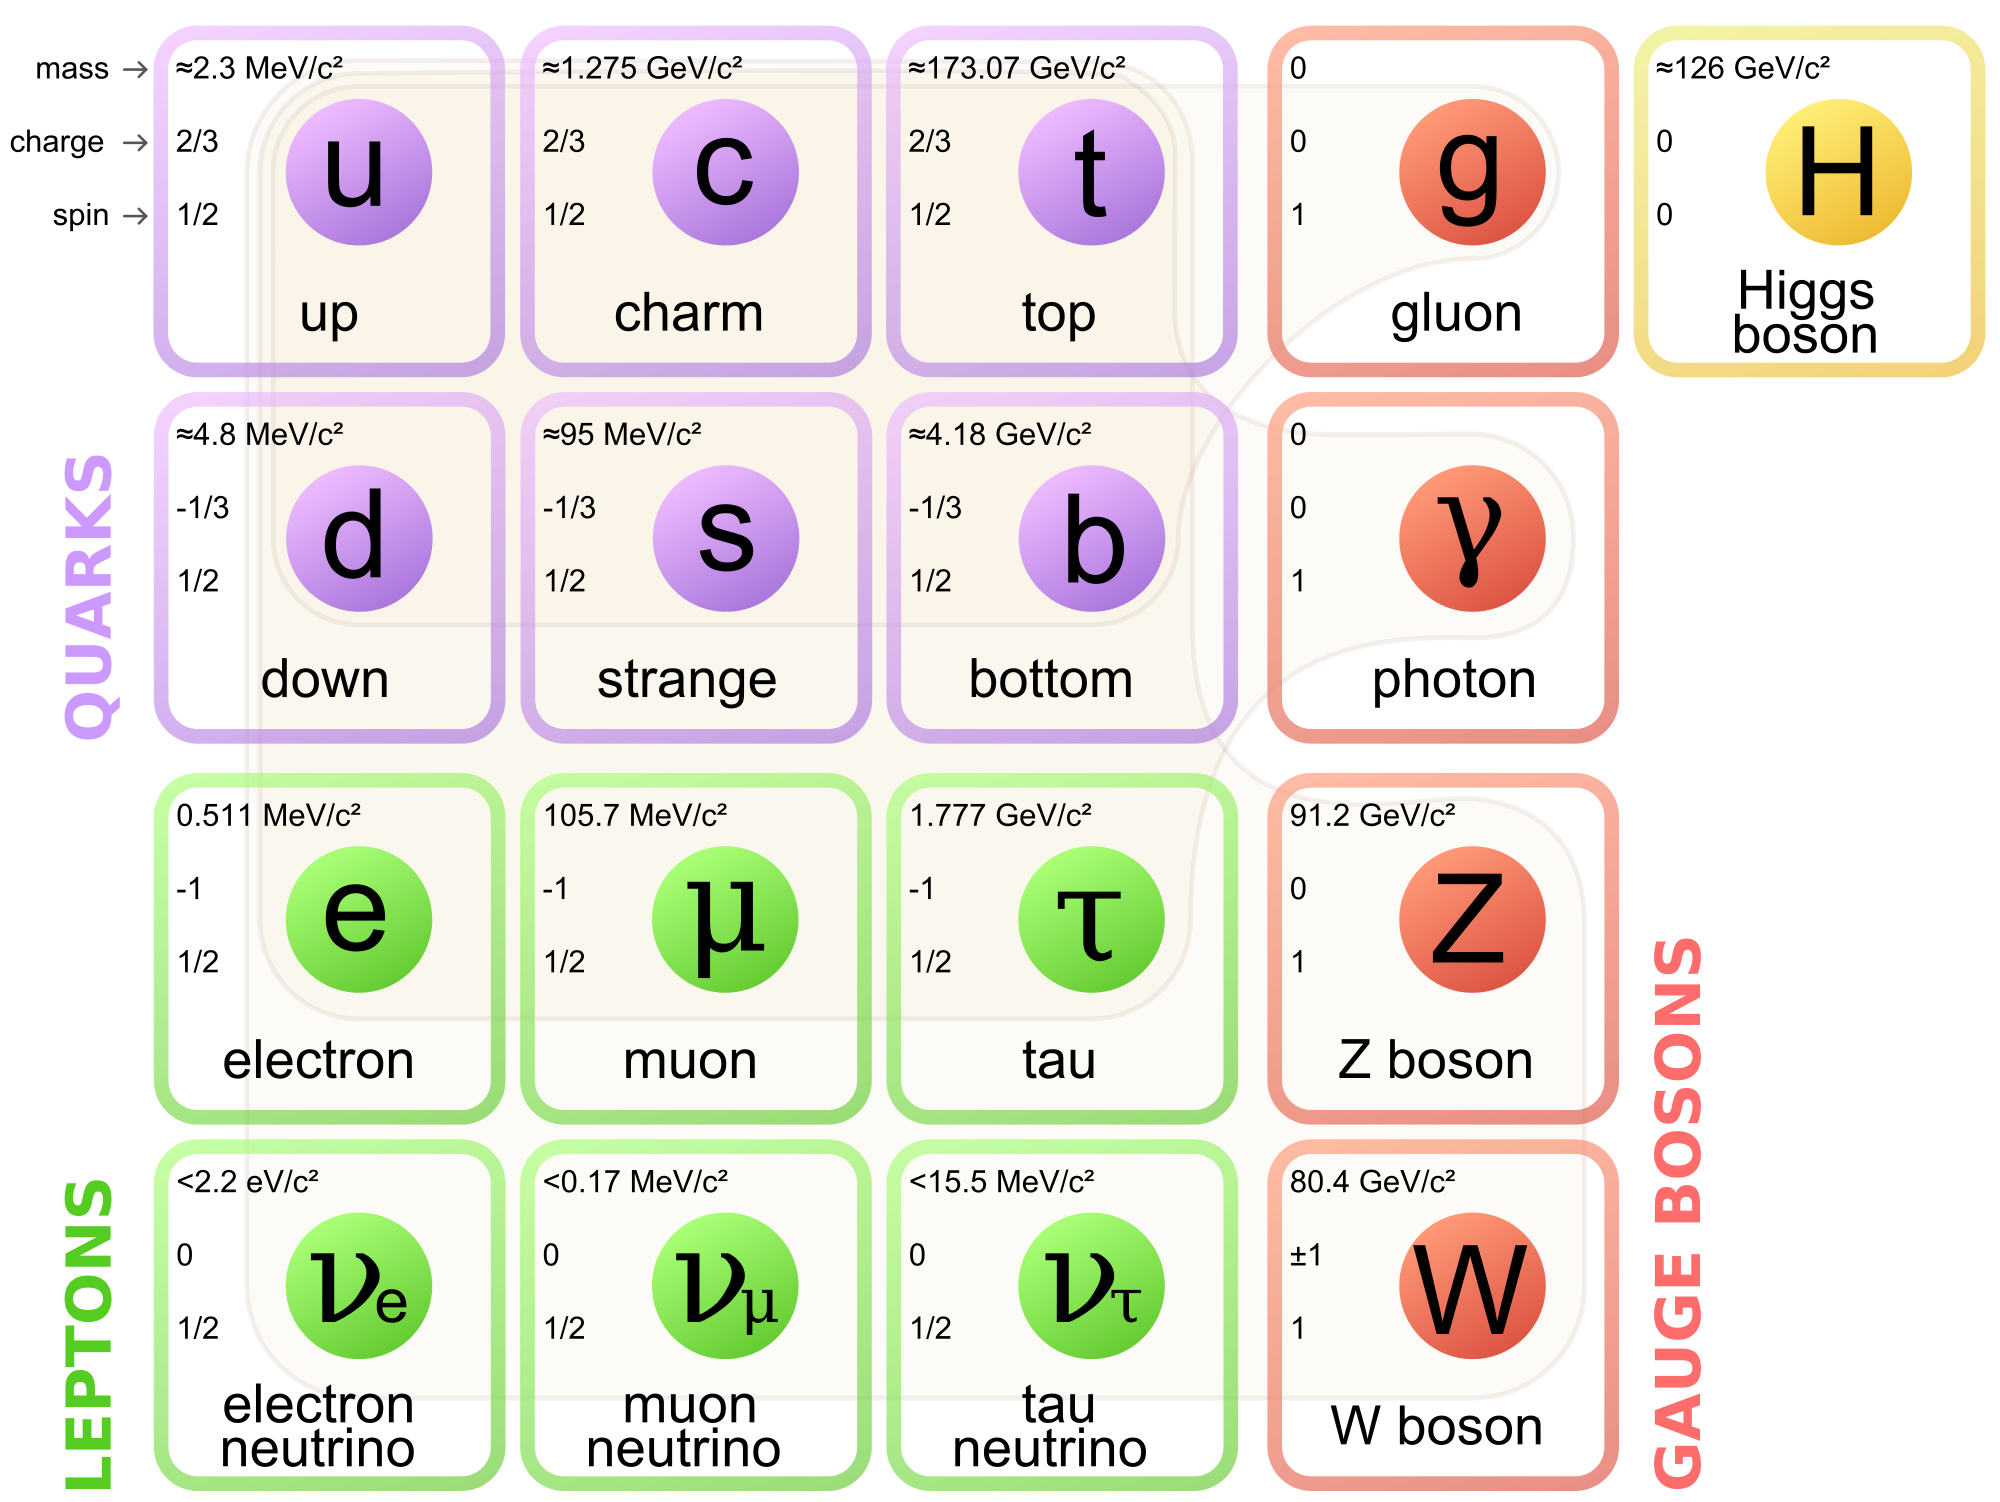
\includegraphics[width=\textwidth]{Chapter1/SM.png} 
  \caption{The system of fundamental particles of the SM. Figure from
    \cite{wiki:SMParticlesSource}}
  \label{fig:SMparticles}
\end{figure}

Quarks bind together to form hadrons and there are hundreds (?source?) of known
hadrons up to date. Theory describing the interaction between quarks is called
Quantum Chromodynamics (QCD) which key features will be discussed in this
chapter. The reasoning for quark existence and for the description their strong
interaction as $SU(3)$ gauge theory will be presented. Running coupling constant
will be discussed to split QCD into perturbative and non-perturbative regions -
two regions, where QCD has to use different mathematical approach for description of
strong interaction. Most of ideas presented here is overtaken from the following
textbook \cite{QCDTextbook}.

\section{Theoretical Ansatz}

In 1950s there have already been discovered tens of new hadrons thanks to new
particle accelerators and a lot of effort was exerted to categorize them. To each
particle there was assigned a series of quantum numbers
including isospin $T$ with its third component $T_3$, hypercharge $Y$,
electrical charge $Q$, strangeness $S$, baryon number $B$ and others. Soon it
was recognized, that there are some symmetries between these quantum numbers,
like Gell-Mann--Nishijima relation \cite{GellMannNishijima1,GellMannNishijima2}

\begin{equation}
  Q = T_3 + 1/2 Y \quad , \quad Y = B + S + \dots,
  \label{ex:GellMannNishijima}
\end{equation}
where dots denotes charm, bottomness and topness. Some of the hadrons known by
then are shown in table \ref{tab:SelectedHadrons}. In 1960s the known particles
were successfully categorized with the so called Eightfold Way, which was
published independently by Murray Gell-Mann (?citace?) and George Zweig
(?citace?) in 1964. The Eightfold Way successfully predicted the existence of new particle
$\Omega^{--}$ including its mass. Basic ideas of Eightfold way will be discussed
in this section.

\begin{table}
  \centering
  \begin{tabular}{|C{1cm}|C{1cm}|C{1cm}|C{1cm}|C{1cm}|C{1cm}|}
    \multicolumn{1}{c|}{} & $S$ & $Y$ & $T$ & $T_3$ & $Q$  \\
    \hline \hline
    $p$ & \multirow{2}{*}{0} & \multirow{2}{*}{1} & \multirow{2}{*}{1/2} & 1/2  & 1 \\
    $n$ &                    &                    &                      & -1/2 & 0 \\
    \hline                                                              
    $\Sigma^+$  & \multirow{4}{*}{-1} & \multirow{4}{*}{0} & \multirow{3}{*}{1} & 1  & 1  \\
    $\Sigma^0$  &                     &                    &                    & 0  & 0  \\
    $\Sigma^-$  &                     &                    &                    & -1 & -1 \\
    $\Lambda$   &                     &                    & 0                  & 0  & 0  \\
    \hline                                                              
    $\Xi^0$ & \multirow{2}{*}{-2} & \multirow{2}{*}{-1} & \multirow{2}{*}{1/2} & 1/2 & 0  \\
    $\Xi^-$ &                     &                     &                      &-1/2 & -1 \\
    \hline
  \end{tabular}
  \caption{Quantum numbers of selected baryons known in 1950s. $S$ strangeness,
  $Y$ hypercharge, $T$ isospin, $T_3$ third component of isospin, $Q$ electrical
charge.}
  \label{tab:SelectedHadrons}
\end{table}

The key feature of Eightfold Way is to understand hadrons as the part of
different representations of infinitesimal generators of $SU(3)$ flavor symmetry
group. Lie algebra of $SU(3)$ is real eight-dimensional Lie algebra
$\mathfrak{su}(3)$ which fundamental representation is usually derived from
Gell-Mann matrices

\begin{align}
  &\lambda_1 = \begin{pmatrix} 0 & 1 & 0 \\ 1 & 0 & 0 \\ 0 & 0 & 0 \end{pmatrix}
  \quad
  \lambda_2 = \begin{pmatrix} 0 & -i & 0 \\ i & 0 & 0 \\ 0 & 0 & 0 \end{pmatrix}
  \quad
  \lambda_3 = \begin{pmatrix} 1 & 0 & 0 \\ 0 & -1& 0 \\ 0 & 0 & 0 \end{pmatrix}
  \nonumber \\
  &\lambda_4 = \begin{pmatrix} 0 & 0 & 1 \\ 0 & 0 & 0 \\ 1 & 0 & 0 \end{pmatrix}
  \quad
  \lambda_5 = \begin{pmatrix} 0 & 0 & -i\\ 0 & 0 & 0 \\ i & 0 & 0 \end{pmatrix}
  \label{eq:GellMannMatrices} \\
  &\lambda_6 = \begin{pmatrix} 0 & 0 & 0 \\ 0 & 0 & 1 \\ 0 & 1 & 0 \end{pmatrix}
  \quad
  \lambda_7 = \begin{pmatrix} 0 & 0 & 0 \\ 0 & 0 & -i\\ 0 & i & 0 \end{pmatrix}
  \quad
  \lambda_8 = \frac{1}{\sqrt{3}} \begin{pmatrix} 1 & 0 & 0 \\ 0 & 1 & 0 \\ 
                                                              0 & 0 & -2 \end{pmatrix}.
  \nonumber
\end{align}

The generators are usually chosen $g_a = \frac{1}{2} \lambda_a$ and obey the
commutation relation $[g_a,g_b]=if_{abc}g_c$ with $f_{abc}$ being structure
constants. Cartan subalgebra of fundamental representation of $\mathfrak{su}(3)$
is generated by $H_1=g_3$ and $H_2=g_8$. The eigenstates of three-dimensional
representation of $\mathfrak{su}(3)$ can be chosen 

\begin{equation}
  u = \begin{pmatrix} 1 \\ 0 \\ 0 \end{pmatrix} \leftrightarrow \left(
    \frac{1}{2}, \frac{\sqrt{3}}{6} \right), \quad
  d = \begin{pmatrix} 0 \\ 1 \\ 0 \end{pmatrix} \leftrightarrow \left(
    - \frac{1}{2}, \frac{\sqrt{3}}{6} \right), \quad
  s = \begin{pmatrix} 0 \\ 0 \\ 1 \end{pmatrix} \leftrightarrow \left(
    0, - \frac{\sqrt{3}}{3} \right), \quad
  \label{eq:RepresentLie3}
\end{equation}
where the eigenvalues to generators of the Cartan subalgebra was assigned $H_1 u
= \frac{1}{2} u$, $H_2 u = \frac{\sqrt{3}}{6} u$ and similarly for $d$ and $s$
eigenstates. These eigenvalues are shown in figure \ref{fig:QuarkTriplet}. Other
important representation of $\mathfrak{su}(3)$ is eight-dimensional adjoint
representation. This representation has the following eigenstates and
corresponding eigenvalues

\begin{figure}[t]
  \centering
  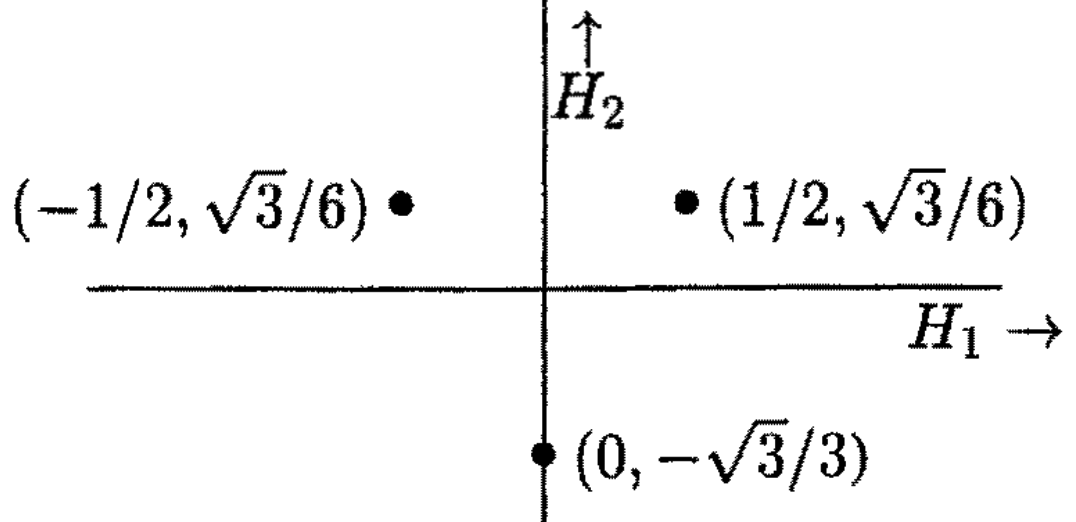
\includegraphics[width=0.5\textwidth]{Chapter1/Quark-triplet.png} 
  \caption{Eigenvalues of 3-dimensional representation of $\mathfrak{su}(3)$ Lie algebra. Figure
    from \cite{LieAlgebrasForParticlePhysicists}.}
  \label{fig:QuarkTriplet}
\end{figure}

\begin{align}
  \frac{1}{\sqrt{2}} \left( g_1 \pm i g_2  \right)
    &\leftrightarrow \left( \pm 1, 0 \right), \nonumber \\
  \frac{1}{\sqrt{2}} \left( g_4 \pm i g_5 \right) 
    &\leftrightarrow \left( \pm \frac{1}{2}, \pm \frac{\sqrt{3}}{2} \right), 
    \label{eq:RepresentLie8} \\
  \frac{1}{\sqrt{2}} \left( g_6 \pm i g_7 \right) 
    &\leftrightarrow \left( \mp \frac{1}{2}, \pm \frac{\sqrt{3}}{2} \right), \nonumber
\end{align}
where again when denoting $A = \frac{1}{\sqrt{2}} ( g_1 + i g_2 )$ then the
upper sign of the first expression reads $[ H_1, A ] = A$ and $[ H_2, A ] = 0$ and
similarly for remaining 5 eigenstates. Defining 

\begin{equation}
  H_1 = T_3 \quad \text{and} \quad H_2 = \frac{\sqrt{3}}{2} Y
  \label{eq:LieIdentification}
\end{equation}
one can easily assign hadrons from table
\ref{tab:SelectedHadrons} to corresponding eigenvalues of adjoint
representation in \ref{eq:RepresentLie8} according to its third component of
isospin $T_3$ and its hypercharge $Y$. This is depicted in figure
\ref{fig:BaryonicOctet}. 

When the same redefinition is done to the eigenstates
of three-dimensional representation in \ref{eq:RepresentLie3}, one can assign to
eigenstates the hypercharge $Y$ and strangeness $S$ as well. The concrete values for
states $u$, $d$, $s$ are shown in table \ref{tab:SelectedQuarks}.

\begin{table}
  \centering
  \begin{tabular}{|C{1cm}|C{1cm}|C{1cm}|C{1cm}|C{1cm}|C{1cm}|}
    \multicolumn{1}{c|}{} & $S$ & $Y$ & $T$ & $T_3$ & $Q$  \\
    \hline \hline
    $u$ & \multirow{2}{*}{0} & \multirow{2}{*}{1/3} & \multirow{2}{*}{1/2} & 1/2
    & 2/3 \\
    $d$ &                    &                      &                      &
    -1/2 & \multirow{2}{*}{-1/3} \\
    $s$ & -1                 & -2/3                 & 0                    & 0    &  \\
    \hline                                                              
  \end{tabular}
  \caption{Quantum numbers of three quarks which existence was predicted by
    Gell-Mann and Zweig in 1964.}
  \label{tab:SelectedQuarks}
\end{table}

\begin{figure}[t]
  \centering
  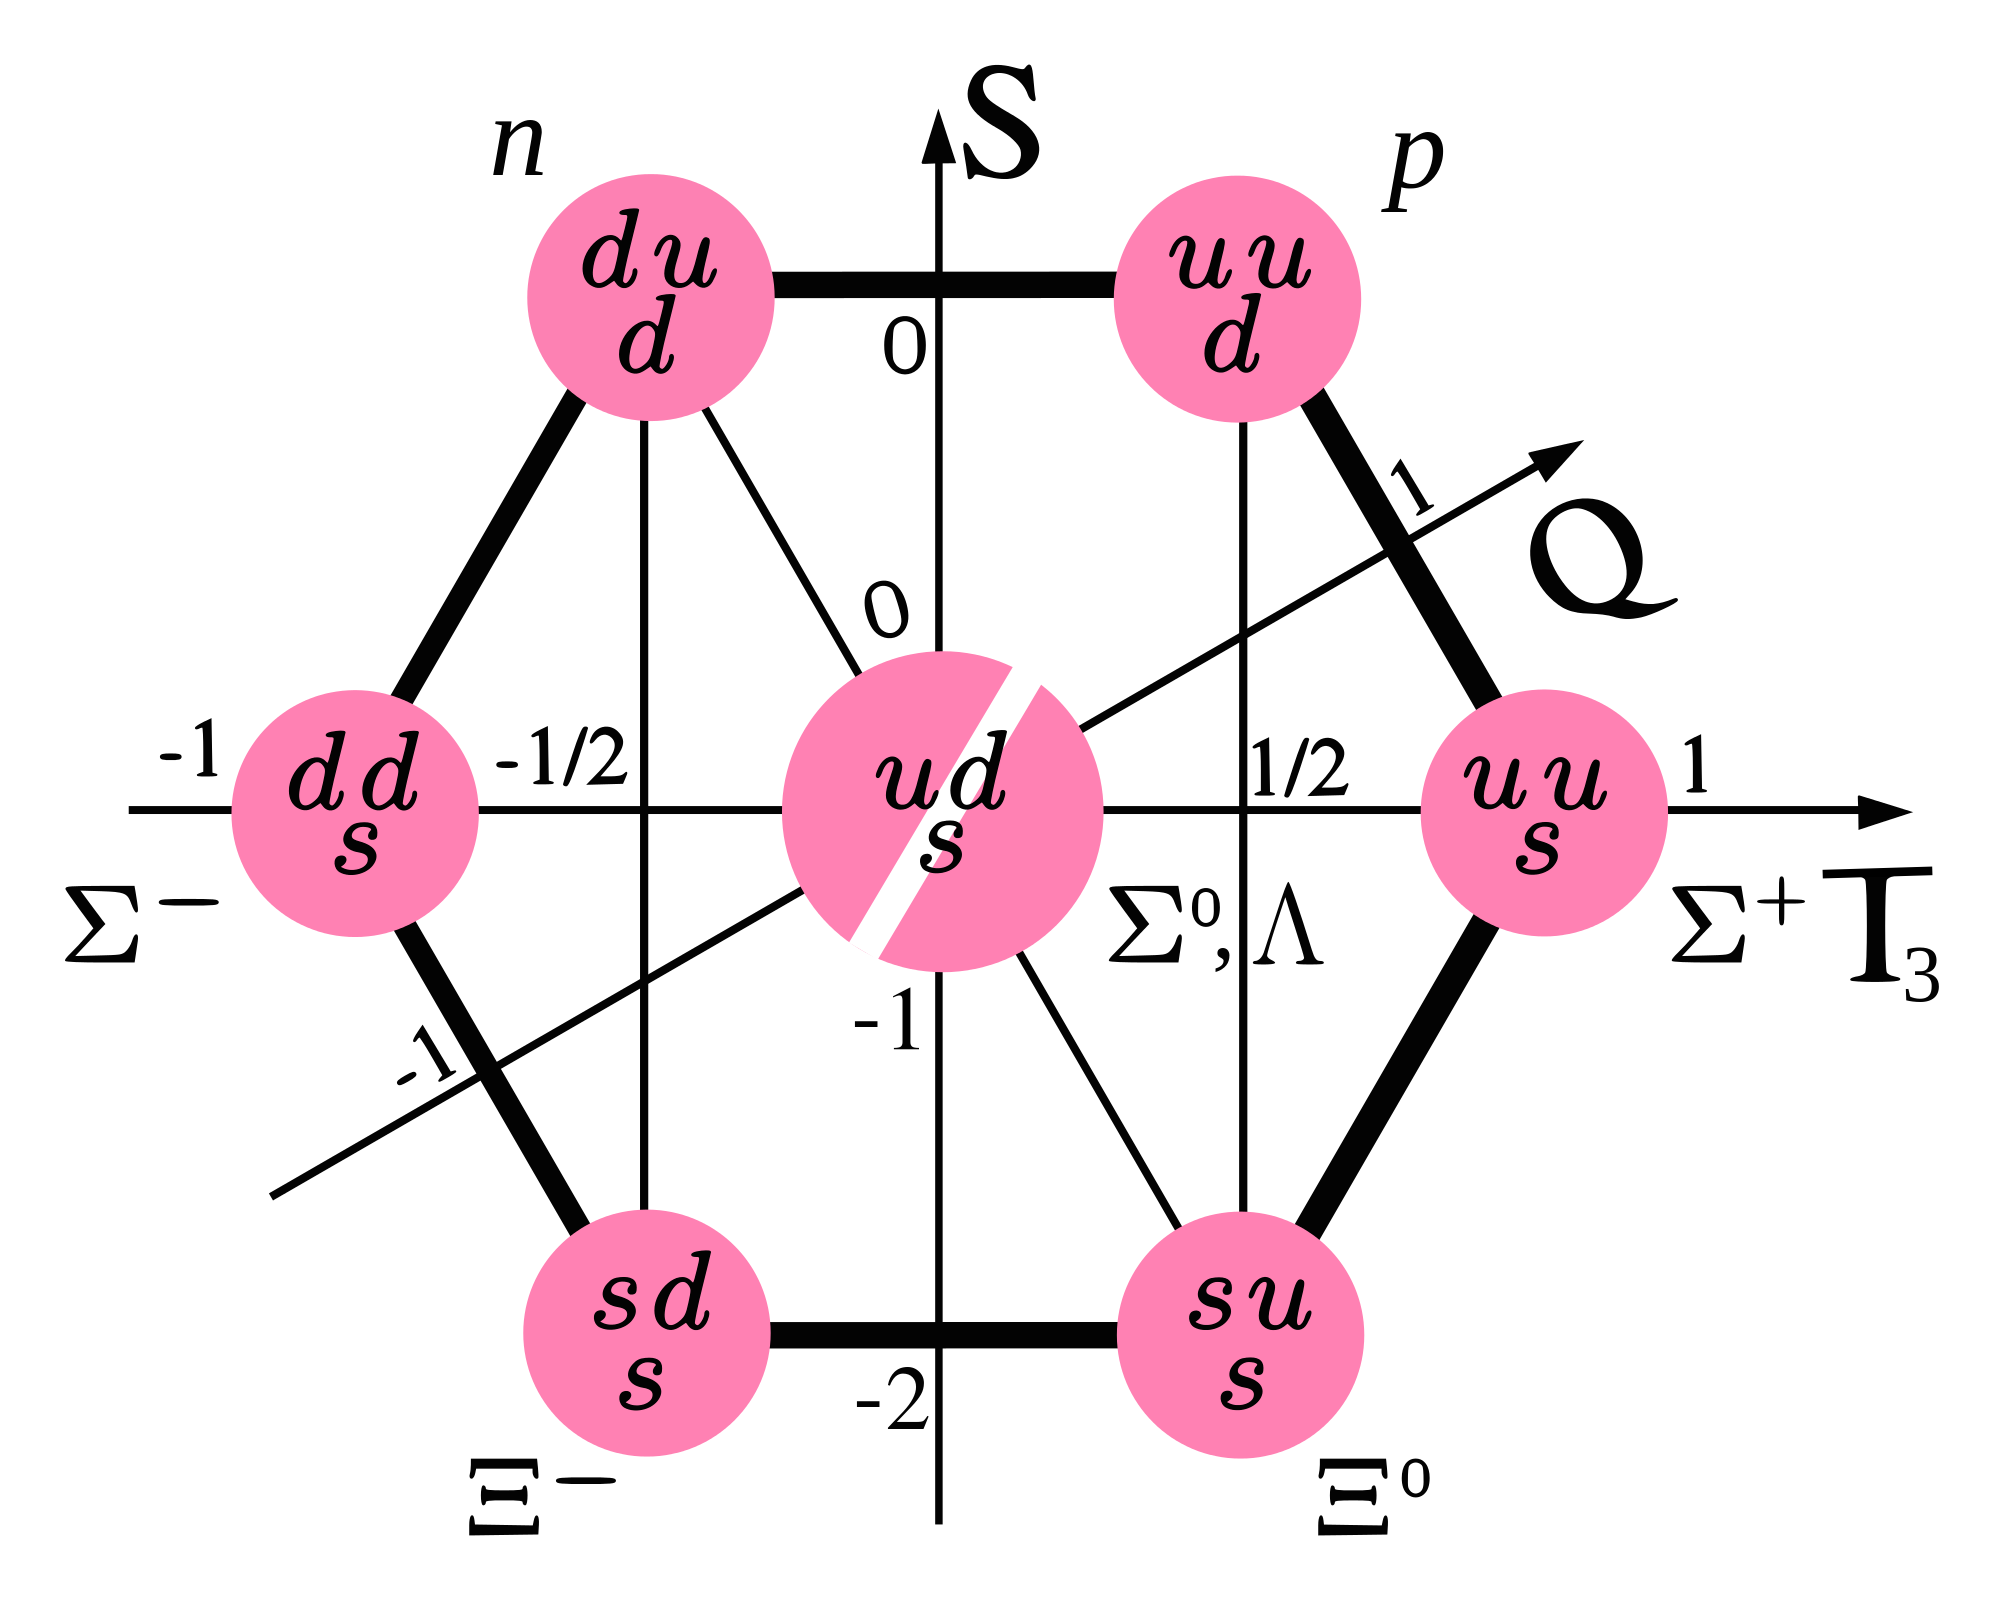
\includegraphics[width=0.5\textwidth]{Chapter1/Baryon-octet.png} 
  \caption{Baryonic octuplet encapsulating baryons from table
    \ref{tab:SelectedHadrons}. For baryons in this diagram, the relation $Y = S
    + 1$ holds. Figure from \cite{wiki:EightFoldWay}.}
  \label{fig:BaryonicOctet}
\end{figure}

It is possible to find another representations of Lie algebra, to which the
observed hadrons can be assigned. The simplest way seems to be through highest
weight defining representation. From eigenvalues of adjoint representation
\ref{eq:RepresentLie8} one can find simple roots 
$\alpha^1=\left( \frac{1}{2}, \frac{\sqrt{3}}{2} \right)$, 
$\alpha^2=\left( \frac{1}{2}, - \frac{\sqrt{3}}{2} \right)$, 
which are defining the highest weights 
$\mu^1=\left( \frac{1}{2}, \frac{\sqrt{3}}{6} \right)$, 
$\mu^2=\left( \frac{1}{2}, - \frac{\sqrt{3}}{6} \right)$.
New representation of Lie algebra can be constructed from highest weight. This
procedure is described in \cite{LieAlgebrasForParticlePhysicists} in detail.

Representations defined by highest weight $\mu^1$ or $\mu^2$ respectively are
called fundamental. Fundamental representation defined by $\mu^1$ is usually
denoted $\mathbf{3}$ and its weight diagram is shown at figure
\ref{fig:QuarkTriplet}, corresponding to three different quark states. The
second fundamental representation corresponds to three anti-quark states and is
usually denoted $\bar{\mathbf{3}}$. Representation depicted in figure
\ref{fig:BaryonicOctet} is defined by the highest weight $\mu^1 + \mu^2$.

Special interest is in representations with dimensions $10$, $8$ and $1$. These
multiplets are present in decompositions $\mathbf{3} \otimes \mathbf{3} \otimes
\mathbf{3} = \mathbf{10} \oplus \mathbf{8} \oplus \mathbf{8} \oplus \mathbf{1}$,
which correspond to the baryons composed of three quarks, and $\mathbf{3}
\otimes \bar{\mathbf{3}} = \mathbf{8} \oplus \mathbf{1}$ corresponding to
mesons from quark and anti-quark.

Important feature of quark model just presented is its capability to predict
hadron masses. This is done using Gell-Mann--Okubo mass formula (?citace?)

\begin{equation}
  M = a_0 + a_1 S + a_2 \left( T(T+1) - \frac{1}{4}S^2 \right),
  \label{eq:GellMannOkubo}
\end{equation}
where $a_0$, $a_1$ and $a_2$ are free parameters which are common for all
hadrons in one multiplet. 

In less than a year after publication of Gell-Mann--Zweig quark model, Sheldon
Lee Glashow and James Bjorken proposed (?citace?) an extension which predicted
existence of fourth flavor of quark - charm quark.

In 1973 the Makoto Kobayashi and Toshihide Moskawa proposed (?citace?) that the
existence of 6 different quark flavors could explain the experimental
observation of CP violation.



\section{Experimental Ground}

\section{QCD as Gauge Theory}

\section{Perturbative QCD}

\section{Non-Perturbative QCD}


\chapter{QCD on ATLAS}

\chapter{ATLAS Detector}
\label{ch:intro}


%================================================================================
% Obrazky
%================================================================================
\clearpage
\listoffigures
\addcontentsline{toc}{chapter}{\listfigurename}


%================================================================================
% Tabulky
%================================================================================
\clearpage
\listoftables
\addcontentsline{toc}{chapter}{\listtablename}


%================================================================================
% Bibliografie
%================================================================================

\clearpage
\bibliographystyle{ieeetr}
\bibliography{bibliography}
\addcontentsline{toc}{chapter}{Bibliography}

\end{document}
